\section{Durchführung}
\label{sec:Durchführung}
\subsection{Energieverlust und Reichweite von Alpha-Strahlung}
Zuerst wird der Versuch wie in \ref{fig:Aufbau} aufgebaut.
Das Präperat ist Americium 241 mit einer Halbwertszeit von $T_{1/2}=\qty{458}{\year}$
Der Abstand zwichen Präperat und dem Halbleiter-Detektor beträgt $d=\qty{6}{\centi\meter}$
Dann wird der Glaszylinder mithilfe der Vakuumpumpe evakuiert.
Aufgenommen wird für die Nummer der detektierten Teilchen innerhalb von 2 Minuten durch den Vielkanalanaylsator.
Zudem wird auch der Kanal eingetragen, bei dem die meisten Teilchen detektiert wurden.
Daraufhin wird in $\delta p=\qty{50}{\milli\bar}$ Schritten der Druck im Glaszylinder varriert und die Messung wiederholt, bis keine Alphateilchen detektiert.
Dies wird genau so nochmal für $d=\qty{5}{\centi\meter}$ durchgeführt.

\begin{figure}
    \centering
    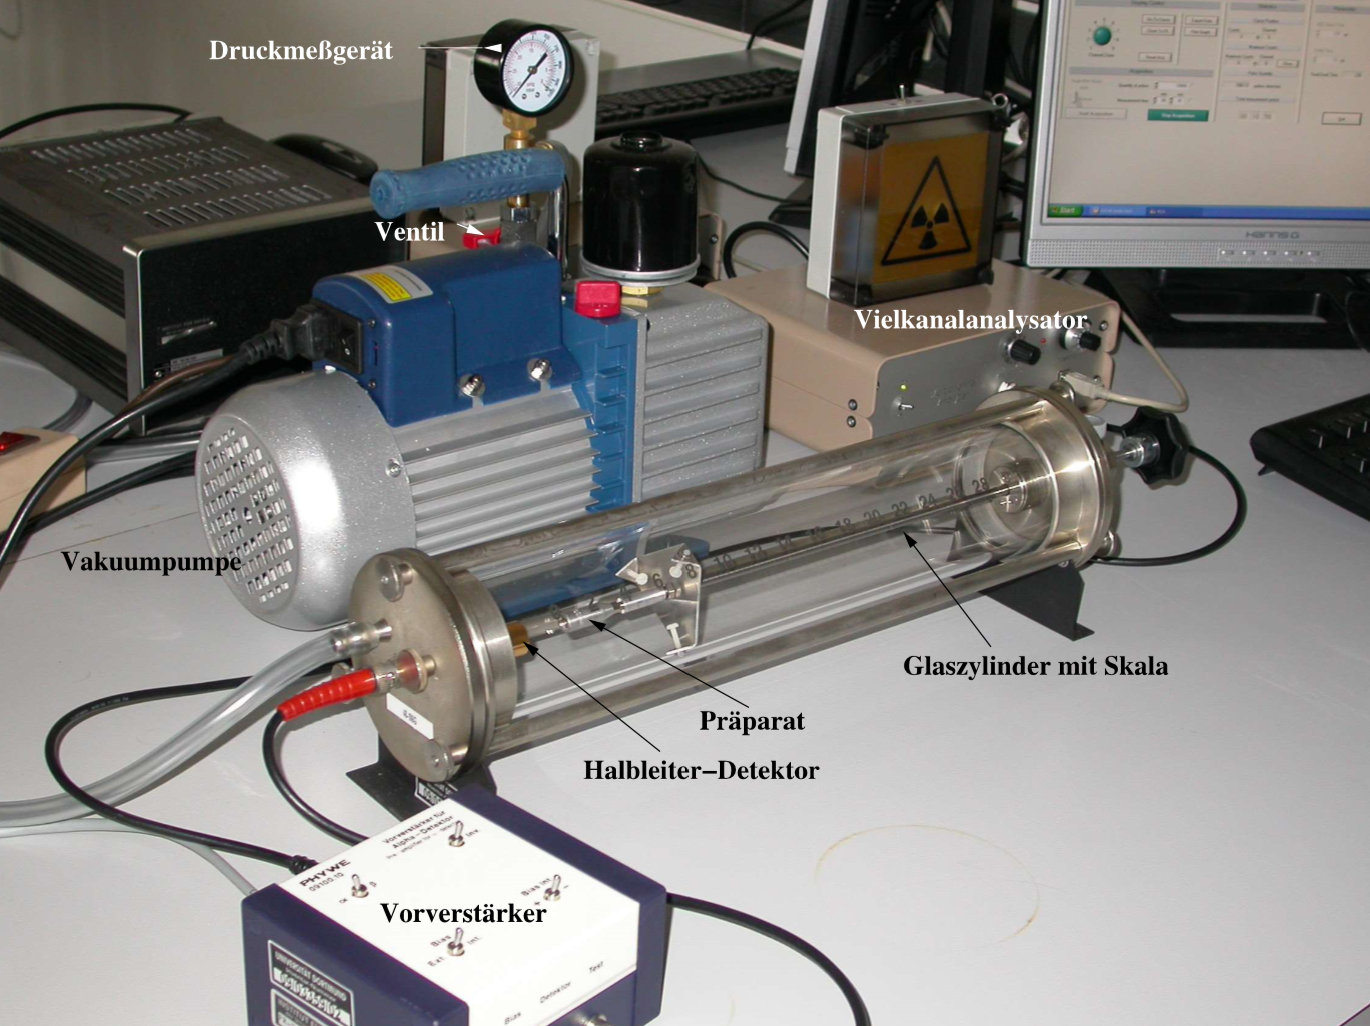
\includegraphics[width=\textwidth]{Bilder/Aufbau.png}
    \caption{Abgebildet ist der Aufbau zur Messung der Energieverteilung der Alphateilchen.}
    \label{fig:Aufbau}
\end{figure}

\subsection{Statistik des radioaktiven Zerfalls}
Es werden 100 Messungen der Anzahl der detektierten Teilchen über einen Zeitraum von 10 Sekunden genommen.